% !TeX root = RJwrapper.tex
\title{GeoAdjust: Adjusting for Positional Uncertainty in Geostatistial Analysis of DHS Data}


\author{by Umut Altay, John Paige, Andrea Riebler, and Geir-Arne Fuglstad}

\maketitle

\abstract{%
The R-package GeoAdjust adjusts for positional uncertainty in GPS
coordinates and performs fast empirical Bayesian geostatistical
inference for household survey data from the Demographic and Health
Surveys (DHS) Program. DHS household survey data is important for
tracking demographic and health indicators, but is published with
intentional positional error to preserve the privacy of the household
respondents. Such jittering has recently been shown to deteriorate
geostatistical inference and prediction, and GeoAdjust is the first
software package that corrects for jittering in geostatistical models
containing both spatial random effects and raster- and distance-based
covariates. The package provides inference for model parameters and
predictions at unobserved locations, and supports Gaussian, binomial
and Poisson likelihoods with identity link, logit link, and log link
functions, respectively. GeoAdjust provides functions that make model
and prior specification intuitive and flexible for the user, as well
as routines for plotting and output analysis.
}

\section{Introduction}

The Demographic and Health Surveys (DHS) Program\footnote{\url{https://dhsprogram.com}} implements household surveys to collect and disseminate nationally representative data about health, population, HIV and nutrition in low- and middle-income countries. The DHS Program started in 1984, and has been implemented in overlapping 5-year phases. So far more than 400 surveys have been conducted in over $90$ countries. Standard DHS surveys usually include between \numprint{5000} and \numprint{30000} households. GPS coordinates of household centres are provided to allow for spatial analyses of the collected demographic and health data, but the DHS has added intentional positional errors into the published GPS coordinates to protect the privacy of the survey respondents \citep{DHSspatial07}.

The random displacement procedure, or \emph{jittering} scheme, is publicly known \citep{DHSspatial07}, but traditional geostatistical analyses assume that the locations are known exactly and ignore the jittering. However, we have recently demonstrated that ignoring the positional error in DHS data may lead to attenuated estimates of the covariate effect sizes and reduced predictive performance \citep{altay2022covariates}. 

While common practice is to ignore jittering, some approaches have been proposed to account for it. With respect to the error induced in spatial covariates, \citet{warren2016influenceOne} proposed regression calibration for distance-based covariates, and \citet{perez2013guidelines,perez2016influence} proposed using a 5 km moving window (or buffer zone) for raster-based covariates. However, these approaches do not address the attenuation arising in the covariate effect sizes when replacing the true covariate with a proxy. With respect to the error induced in the spatial effect, \citet{fanshawe2011spatial} proposed a Bayesian approach in the limited setting of no covariates and Gaussian observation model. \citet{wilson2021estimation} proposed a more complex approach using INLA-within-MCMC \citep{rue2009approximate, gomez2018markov}, which could handle the error induced in both the spatial random effect and in spatial covariates, but computation time is too extensive for routine use of the approach. None of the mentioned papers provide an R package for easy application of the methods.

The datasets from DHS are semi-public and one must apply for access. A step-by-step explanation of the application procedure can be found at \url{https://dhsprogram.com/data/new-user-registration.cfm}. The application requires a brief project description  explaining why the data set is needed and how it will be used. Permission is typically granted within a few days.

With the R package \CRANpkg{GeoAdjust}, we address the need for fast, flexible and user-friendly software to estimate geostatistical models for DHS data subject to positional uncertainty. \CRANpkg{GeoAdjust} corrects for the positional uncertainty by adjusting for jittering both in the spatial random effect and the spatial covariates, and achieves fast inference by combining the computational efficiency of the stochastic partial differential equations (SPDE) approach \citep{Lindgren:etal:11} with the autodifferentiation features of Template Model Builder (TMB) \citep{tmb}. We use the R-package \CRANpkg{fmesher} \citep{fmesherPackage} for computing the mesh and discretization matrices for the SPDE approach, and the R-package \CRANpkg{TMB} for easy use of the TMB methodology. \CRANpkg{GeoAdjust} is available on CRAN \citep{Rmain} and can be installed with the command \code{install.packages("GeoAdjust")}. While there are other R packages such as \CRANpkg{SUMMER} \citep{li2020space,summerPackage} that can perform spatial or spatio-temporal areal analysis of DHS data, none can account for jittering in geostatistical analysis.



\section{Geostatistical inference under jittering}
\label{sec:method}
We describe a country of interest as a spatial domain $\mathcal{D}\subset\mathbb{R}^2$, and we assume that $C$ small groups of households, called \emph{clusters}, are observed within the country. For clusters $c = 1, \ldots, C$, we denote the true location by $\boldsymbol{s}_c^* \in\mathcal{D}$, and we denote the observed (jittered) location, provided by DHS surveys, by $\boldsymbol{s}_c \in\mathcal{D}$. Additionally, each cluster has a known classification as urban (U) or rural (R). The urban/rural designation, $\mathrm{Urb}[c]\in\{\mathrm{U},\mathrm{R}\}$, is important since DHS surveys use different jittering mechanisms in urban and rural clusters.
Urban clusters are jittered up to $2\, \mathrm{km}$, and rural clusters are jittered up to $5\, \mathrm{km}$ with probability $0.99$ and jittered up to $10\, \mathrm{km}$ with probability $0.01$ \citep{DHSspatial07}. The angle and jittering distance are sampled from uniform distributions, but the boundaries of either the first or the second administrative level are respected. We denote these \emph{known} jittering distributions by $\pi_{\mathrm{Urb}[c]}(\boldsymbol{s}_c|\boldsymbol{s}_c^*)$, $c = 1, \ldots, C$.

An observation $y_c$ is made at each cluster $c$, and the responses $y_1, \ldots, y_C$ and the observed locations $\boldsymbol{s}_1, \ldots, \boldsymbol{s}_C$ are modelled jointly as
\begin{align}
y_c \mid \mu_c, \boldsymbol{\phi} &\sim \pi(y_c \mid \mu_c, \boldsymbol{\phi}),  \quad \boldsymbol{s}_c|\boldsymbol{s}_c^*\sim \pi_{\mathrm{Urb}[c]}(\boldsymbol{s}_c|\boldsymbol{s}_c^*), \quad c  = 1, \ldots, C, \label{eq:model}
\end{align}
where  $\pi(y_c \mid \mu_c, \boldsymbol{\phi})$ denotes the likelihood of $y_c$ given the mean $\mu_c$ and the vector of likelihood parameters $\boldsymbol{\phi}$. The intuition is that the observed response $y_c$ and the observed location $\boldsymbol{s}_c$ are independent random variables, which differ from the mean $\mu_c$ and the true location $\boldsymbol{s}_c^*$, respectively.  The mean is linked to a linear predictor $\eta_c$ through a link function $g$ as
\[
    g(\mu_c) = \eta_c.
\]
The package implements the identity link in the case of a Gaussian likelihood, the log-link for Poisson likelihood, and the logit-link for the binomial likelihood. 

We model latent spatial variation in a traditional way as
\[
    \eta(\boldsymbol{s}^*) = \boldsymbol{x}(\boldsymbol{s}^*)^\mathrm{T}\boldsymbol{\beta}+u(\boldsymbol{s}^*), \quad \boldsymbol{s}^* \in\mathcal{D},
\]
where $\boldsymbol{x}(\cdot)$ is a vector of $p$ spatial covariates, $\boldsymbol{\beta}$ is a vector of $p$ coefficients, and $u(\cdot)$ is a Matérn Gaussian random field (GRF). The GRF $u(\cdot)$ is controlled by the three parameters: smoothness $\nu$, which is fixed to 1, spatial range $\rho_\mathrm{S}$, and marginal variance $\sigma_\mathrm{S}^2$. The key difference from a standard geostatistical model is that the mean
\[
    \mu_c = g^{-1}(\eta_c) = g^{-1}(\eta(\boldsymbol{s}_c^*))
\]
 depends on the \emph{unknown} true location $\boldsymbol{s}_c^*$. This means that we do not know from which pixel to extract covariates and we do not know at which location to evaluate the GRF.

We choose a uniform prior $\boldsymbol{s}_c^*\sim \mathcal{U}(\mathcal{D})$ for the true cluster location, implying that all $\boldsymbol{s}_c^*$ compatible with $\boldsymbol{s}_c$ are equally likely \emph{a priori}, $c = 1, \ldots, C$.  In the case of Nigeria, which is the country used as an example in later sections, compatible refers to all potential true cluster locations lying in the same second administrative area (admin2) as the observed location and within the maximum jittering distance. More complicated priors that take population density or urban/rural status into account are possible, but such rasters would have to be estimated and could be biased and uncertain.
Further, $\boldsymbol{\beta}\sim\mathcal{N}_p(\boldsymbol{0},V \mathbf{I}_p)$, where $V$ is a fixed variance, and $\rho_\mathrm{S}$ and $\sigma_\mathrm{S}^2$ are assigned penalized complexity (PC) priors with $\mathrm{P}(\rho_\mathrm{S} > \rho_0) = 0.50$ and $\mathrm{P}(\sigma_\mathrm{S} > 1) = 0.05$ \citep{fuglstad:etal:19a}. We recommend choosing the median range $\rho_0$ as 10\% of the diameter of $\mathcal{D}$ to be able to capture the spatial variability at moderate distances. 

For inference, \CRANpkg{GeoAdjust} treats the unknown true locations as nuisance parameters and integrates them out,
\begin{align}
    \pi(y_c, \boldsymbol{s}_c|\eta(\cdot)) &= \int_{\mathcal{D}} \pi(y_c, \boldsymbol{s}_c| \eta(\cdot), \boldsymbol{s}_c^*) \pi(\boldsymbol{s}_c^*) \ \mathrm{d}\boldsymbol{s}_c^* \notag \\
    &= \int_{\mathcal{D}} \pi(y_c| \eta(\boldsymbol{s}_c^*)) \pi_{\mathrm{Urb}[c]}(\boldsymbol{s}_c| \boldsymbol{s}_c^*) \pi(\boldsymbol{s}_c^*) \ \mathrm{d}\boldsymbol{s}_c^*.\label{eq:numInt}
\end{align}
This means that the likelihood of $y_c$ is considered to be a mixture distribution over all true locations $\boldsymbol{s}_c^*$ compatible with the observed location $\boldsymbol{s}_c$, where the weighting is informed by the prior and the known jittering mechanism.
In the implementation, the integral is computed numerically  using a integration scheme constructed with rings of integration points centered around the DHS provided cluster location $\boldsymbol{s}_c$. Hence, Equation \eqref{eq:numInt} is approximated by a finite mixture over potential true locations. 
Computational efficiency is achieved by combining the SPDE approach \citep{Lindgren:etal:11} to describe $u(\cdot)$ and TMB which allows for fast and flexible autodifferentiation. For details on the the integration scheme and the inference scheme, we refer to \citet{altay2022accounting,altay2022covariates}.

\section{Package structure and functionality}
\CRANpkg{GeoAdjust} handles the technical steps of the method described in the previous section in order to make the adjustment for jittering widely accessible.  Figure \ref{fig:workflow} illustrates the structure of \CRANpkg{GeoAdjust}, and how various data inputs are processed through the package workflow. The main functionality of the package is described below, and is broken down into the three main steps of the workflow illustrated in Figure \ref{fig:workflow}: input preparation, estimation, and prediction.

\begin{figure}
\centering
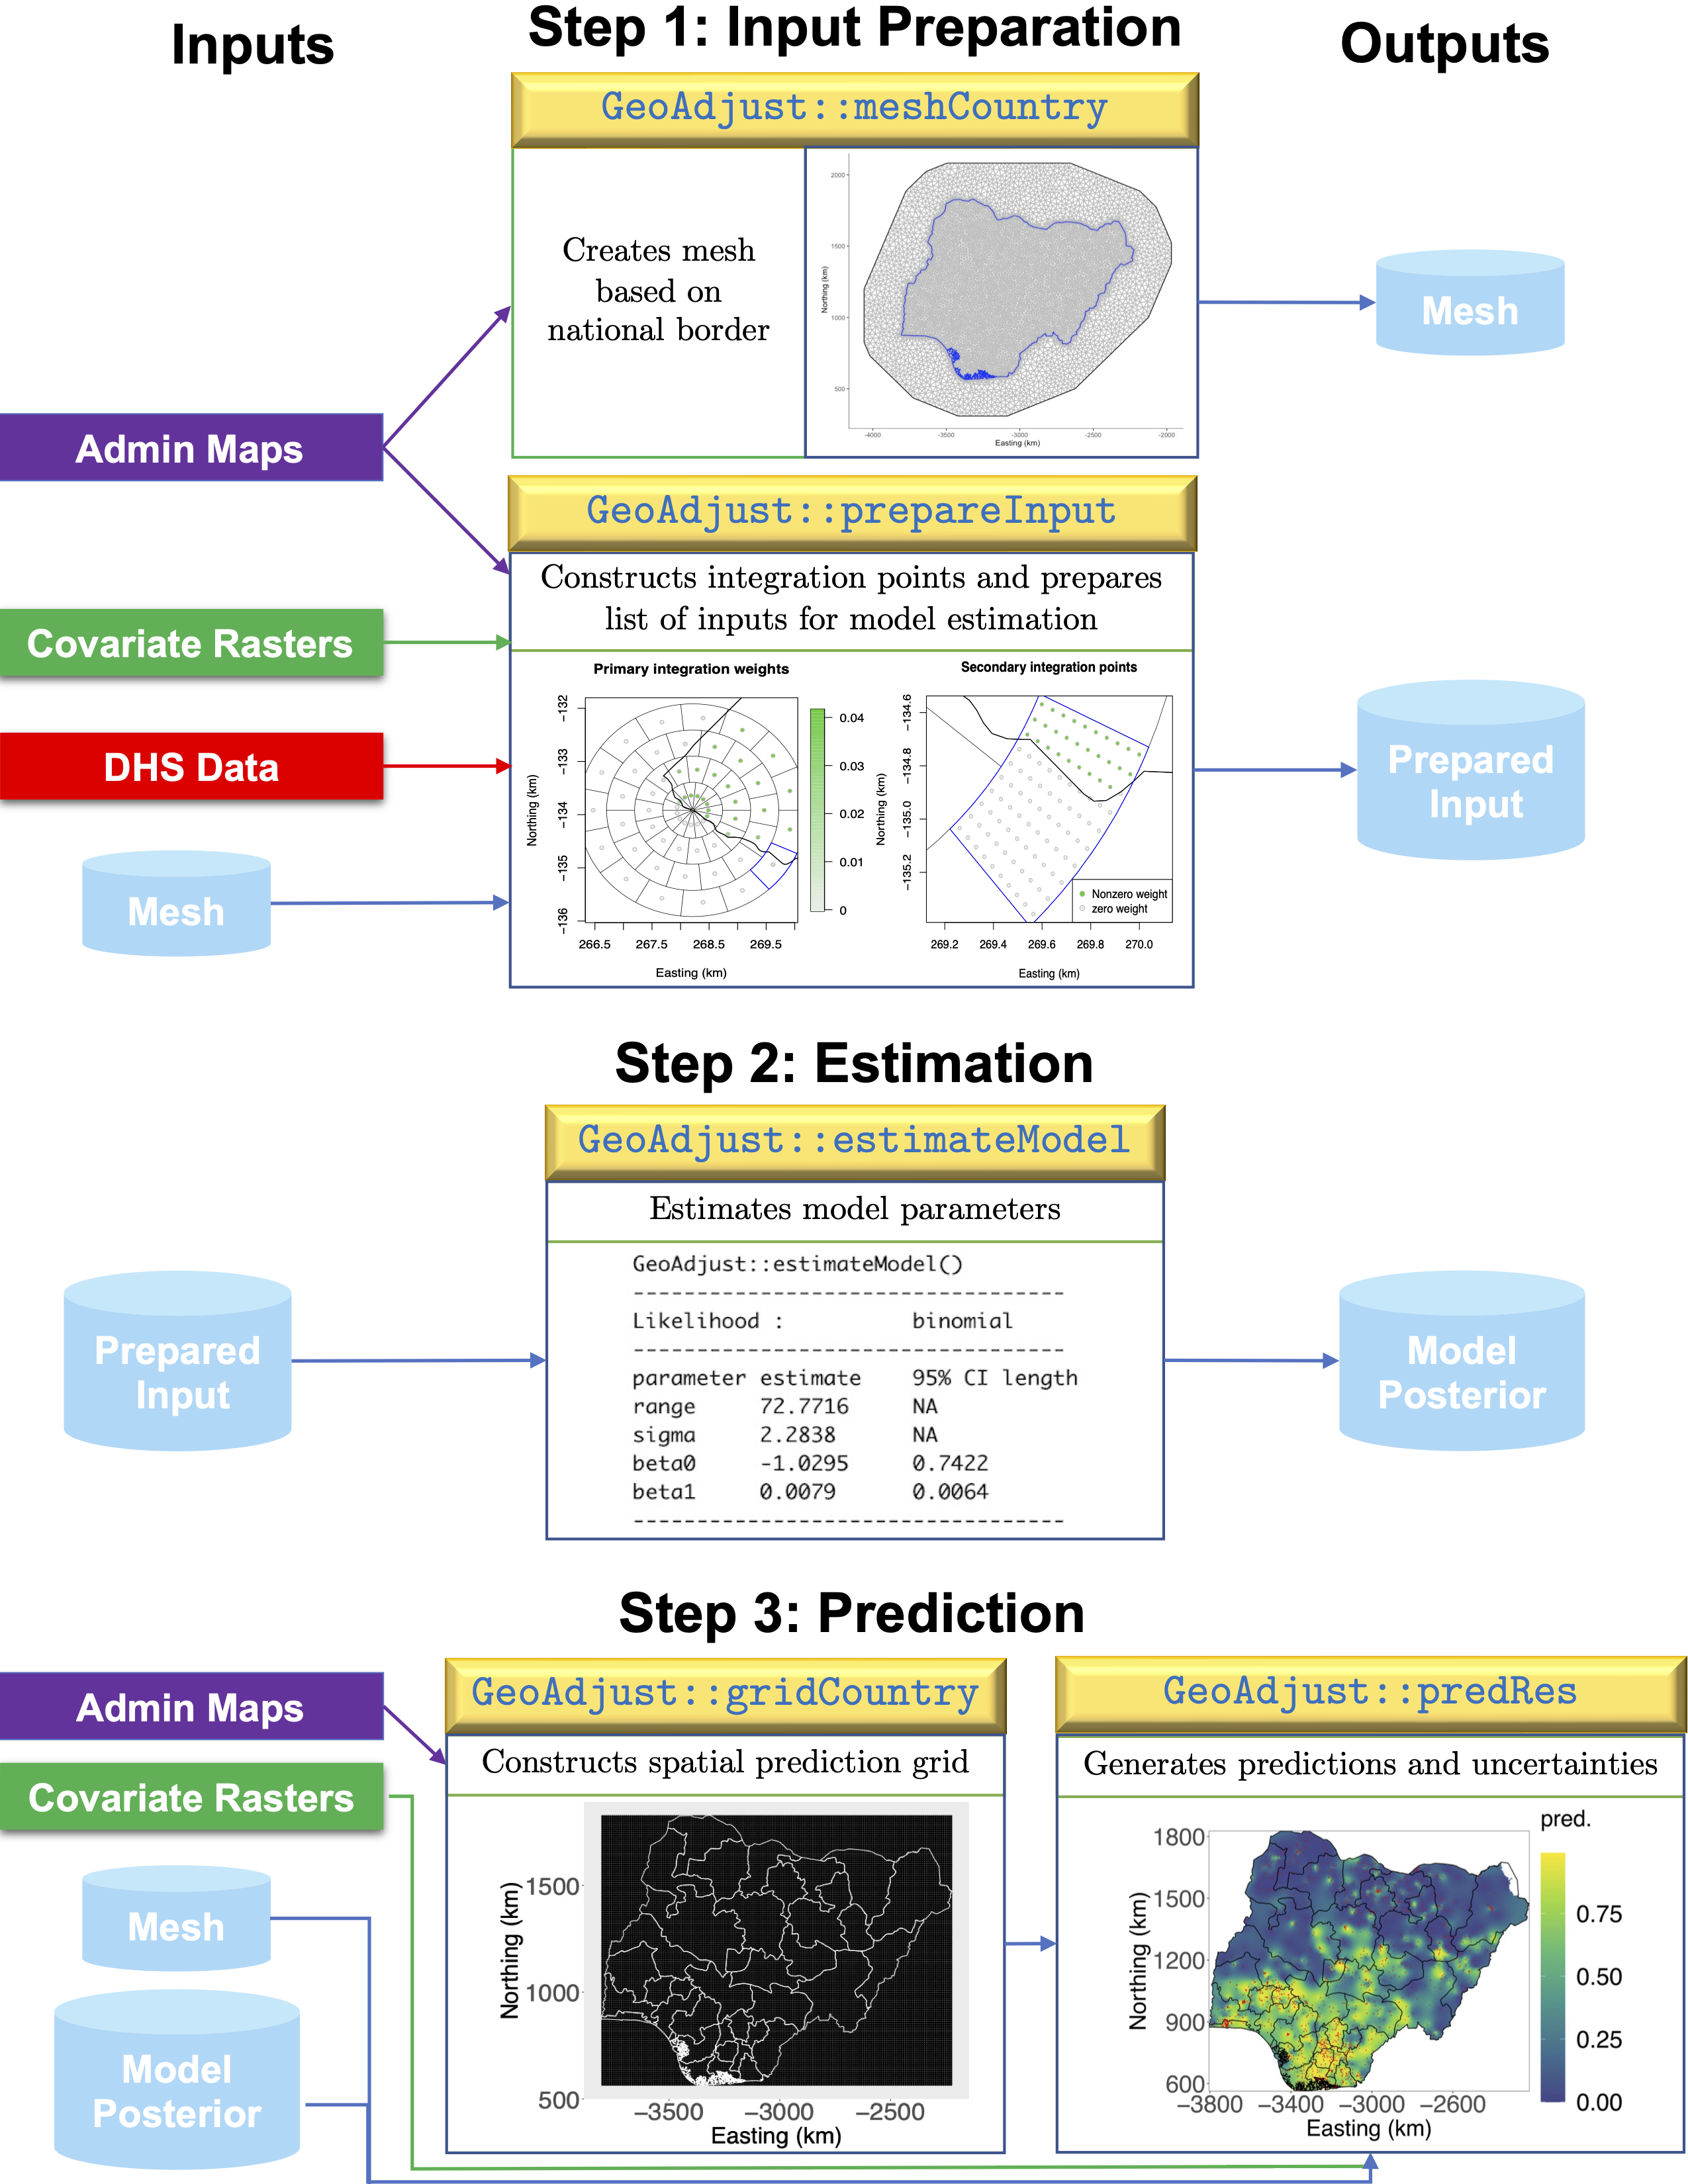
\includegraphics[width=\textwidth]{workflowVert.png}
\caption{A visual representation of \CRANpkg{GeoAdjust} workflow.}
\label{fig:workflow}
\end{figure}

\subsection{Step 1: Input preparation \label{sec:InputPreparation}}
Before estimation and prediction, \CRANpkg{GeoAdjust} requires a set of triangular basis functions forming a `mesh' that is necessary for the SPDE approach, and also a separate data structure containing relevant information about the input datasets and the jittering. \CRANpkg{GeoAdjust} facilitates the preparation of these inputs via the functions \code{meshCountry} and \code{prepareInput}.
%\subsection{Mesh generation for the region under study \label{sec:Triangulation}}
In \CRANpkg{GeoAdjust}, the GRF $u(\cdot)$ is approximated using the so-called SPDE approach. This requires the construction of a constrained refined Delaunay triangulation (CRDT), a mesh over the country of interest. The approximated spatial field can then be projected from the mesh nodes to the cluster centers via projector matrices \citep{Lindgren:etal:11}. The function \texttt{meshCountry}  creates a triangular mesh based on the national borders.
It has five arguments: \texttt{max.edge} is a vector of two values, where its first and second elements represent the largest allowed triangle edge lengths for the inner and outer mesh, respectively, and \texttt{offset} stands for the extension distance outside the country borders. A negative value is interpreted as a relative extension, e.g., $-0.08$ means an extension of 8\%. The argument \texttt{admin0} is an \CRANpkg{sf} (simple features) object of class \texttt{MULTIPOLYGON} containing the geometry of the national borders of the country, \texttt{cutoff} is the minimum allowed distance of the vertices to each other \citep{fmesherPackage}, and \code{target\_crs} describes the coordinate reference system (CRS) that the function operates within. The CRS string is set by the user based on where on earth the user wishes to do their modeling, since different projections are intended for use in different parts of the world.
See Step 1 in the Nigeria example for a demonstration.

%\subsection{Input data preparation}
The integration in Equation \eqref{eq:numInt} is performed numerically. To calculate the integrals, we need a set of integration points around the associated jittered survey cluster centers. \CRANpkg{GeoAdjust} specifies the cluster center itself as the first integration point and builds either 5 or 10 rings around it, depending on whether it is located in an urban or a rural stratum, respectively. Each ring contains a set of 15 angularly equidistant `primary' integration points as illustrated in the left panel of Figure \ref{fig:intPtIllustration}.
The first 5 rings are called the "inner rings". An additional 5 rings are constructed for the rural cluster centers, and are called the "outer rings". The primary integration points are assigned equal weight \textit{a priori} within any single ring, where the weight for a given ring is determined by the jittering distribution. Weights of individual points are adjusted, however, for relevant subnational boundaries. If an observed cluster location is closer to the nearest relevant subnational border than the maximum jittering distance, a set of secondary integration points are constructed, each with an associated primary integration point, and the weight of each primary integration point is distributed among the associated secondary integration points. Zero weight is assigned to any secondary integration points that are across the border, and weights are then reaggregated to the primary integration points to create the final integration weights of the primary integration points. Figure \ref{fig:intPtIllustration} shows an example set of primary and secondary integration points and the corresponding integration weights for a single cluster from the Kenya 2014 DHS household survey. The supplementary materials of \citep{altay2022accounting} provides a detailed mathematical explanation of the procedure.

\begin{figure}
\centering
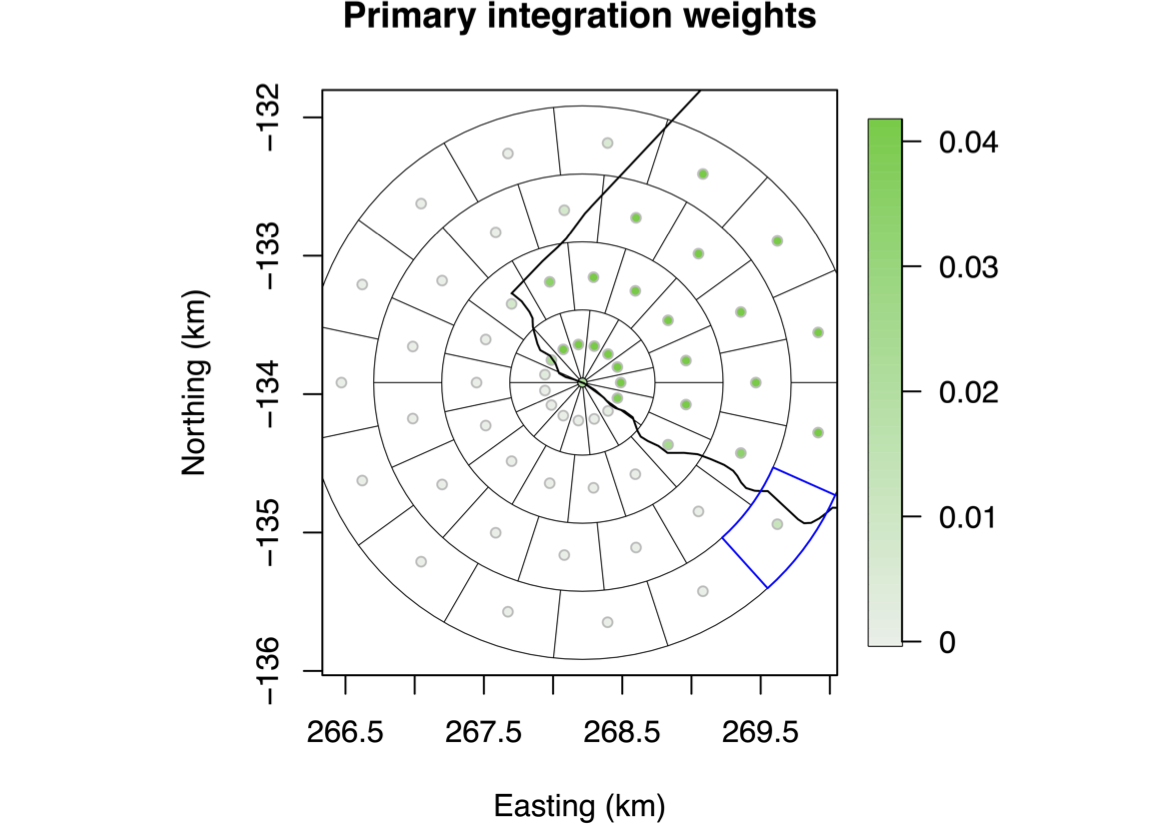
\includegraphics[width=.49\textwidth]{intPtIllustration.png} 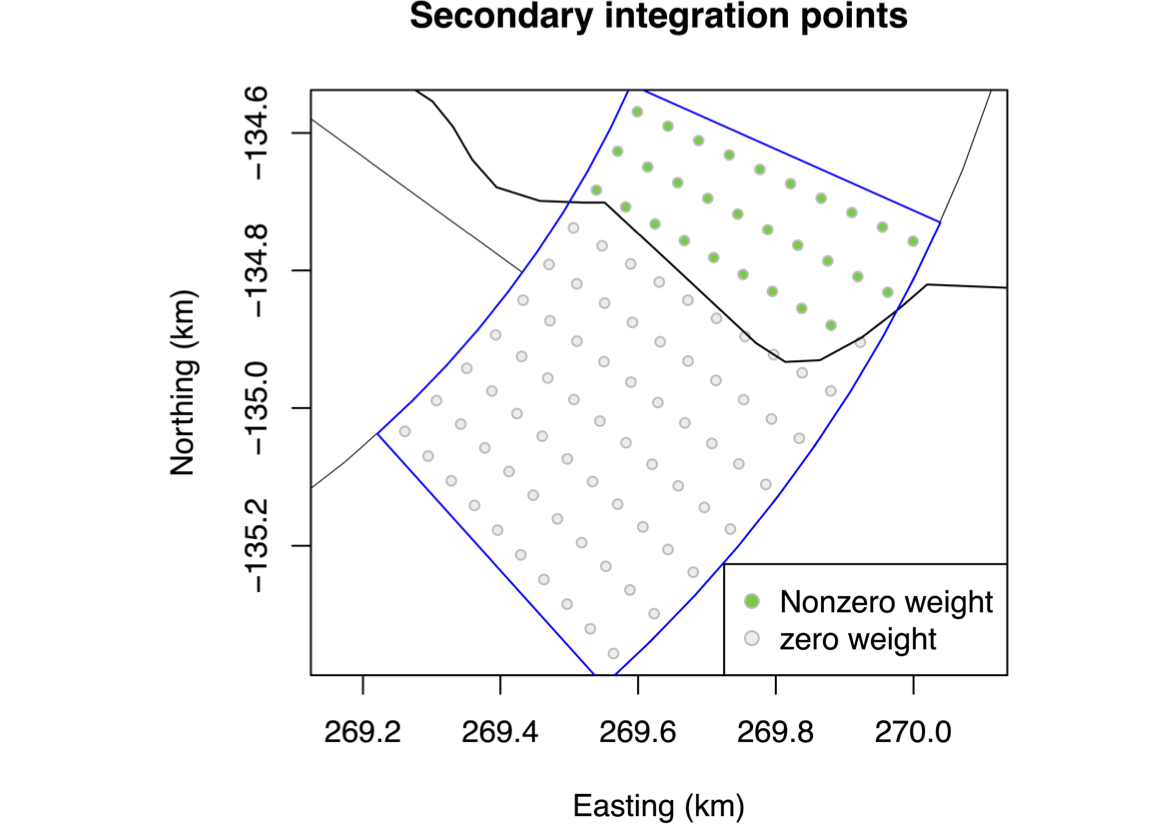
\includegraphics[width=.49\textwidth]{subIntPtIllustration2.png}
\caption{Illustration of primary (left) and secondary (right) integration weights for one cluster from Kenya 2014 DHS household survey.}
\label{fig:intPtIllustration}
\end{figure}

 The function \code{prepareInput} creates the set of integration points and weights with respect to the urban/rural strata, and constructs the urban and rural design matrices by extracting the covariate values at each integration point. Internally, \code{prepareInput} function conducts various distance based calculations and comparisons, all measured in kilometers. Therefore, the measurement unit of the \code{target\_crs} \strong{must} also be in kilometers.
The output of \code{prepareInput} is a list containing the strata-wise design matrices and response vectors, together with the sparse matrix components of the SPDE model, and strata-wise projector matrices.  The argument \code{likelihood} can be \code{0} (Gaussian), \code{1} (Binomial), and \code{2} (Poisson). For the Gaussian and Poisson likelihoods, the argument \code{response} contains a list containing a vector \code{ys} containing observed values, and, for the Binomial likelihood, the argument \code{response} contains a list with a vector \code{ns} with the number of trials and a vector \code{ys} with the number of successes. See Step 1 in the Nigeria example for a demonstration.

\subsection{Step 2: Estimation}
The list returned by the \texttt{prepareInput} function described in the previous section contains elements that will be processed by TMB in \texttt{estimateModel}. 
The \texttt{estimateModel} function is a wrapper function built around C++ code implementing our model in TMB, allowing the user to estimate model parameters and to use TMB's autodifferentiation features without needing to know or program in C++. The main argument of \texttt{estimateModel} is a list called \texttt{data}, referring to the input list that has been created by \texttt{prepareInput} function. The function also allows different prior choices for the model components, via its argument called \texttt{priors}. 

The \texttt{priors} argument allows the user to specify the parameters of the Gaussian prior for covariate effect sizes, and of the penalized complexity (PC) priors for the spatial range. These values can be passed into the function as a list of two elements, namely, \texttt{beta} and \texttt{range}. 
The element \texttt{beta} needs to be a vector of length two. The first and the second elements of the vector \texttt{beta} are the mean and the standard deviation of the Gaussian priors that are assigned for the intercept and the covariate effect sizes. The element \texttt{range} refers to the \emph{a priori} median range. Further, the PC priors for marginal variance and measurement variance are passed as \texttt{Uspatial}, \texttt{alphaSpatial}, \texttt{UNugget}, and \texttt{alphaNug}. \texttt{USpatial} is the upper \texttt{alphaSpatial} percentile of the marginal standard deviation, and \texttt{UNugget} and \texttt{alphaNug} are the hyperparameters for the PC-prior on the nugget variance. The hyperparameters \texttt{UNugget} and \texttt{alphaNug} pass into the function as 1 and 0.05, by default, but they are only used in the calculations when the likelihood is Gaussian. 
See Step 2 in the Nigeria example for a demonstration.


Parameter estimation and model fitting via \texttt{estimateModel} integrates out the unknown true coordinates by computing the contribution of each integration point to the joint negative log-likelihood. 
Internally, once the TMB function \texttt{MakeADFun} constructs the core model object \citep{kaskr2022}, \texttt{estimateModel} inputs the objective function and its gradient into the optimization routine, \texttt{optim}. Afterwards, \texttt{estimateModel} extracts the estimated model parameters from the optimized core model object, and draws \texttt{n.sims} posterior samples. This includes samples of the intercept, each covariate effect, and the spatial random effect coefficients for each mesh node as well. The samples for the intercept and the covariate effect sizes are then used for constructing the 95\% credible interval lengths as the measure of uncertainty corresponding to the estimated parameters.

The function \texttt{estimateModel} returns a list of four elements. The list contains a data frame of the estimated model parameters, together with the optimized core model object, a matrix containing the \texttt{n.sims} posterior samples, and information about the type of the likelihood. The core model object and the posterior draws can then be passed to the function \texttt{predRes} to generate predictions at a set of prediction locations. The object returned by \code{estimateModel} can be printed in a tidy way using \code{print}. See Step 2 in the Nigeria example for a demonstration.

\subsection{Step 3: Prediction}
Once the model parameters are estimated, the model can be used for predicting the model outcomes at a new set of locations. The function \texttt{gridCountry} in \CRANpkg{GeoAdjust} helps with the construction of a set of prediction points. The function creates a \texttt{SpatRaster} of the desired resolution within the bounding box of the national level shape file, extracts the coordinates of the cell centers and returns them as an \texttt{sf} class \texttt{POINT} object together with the raster, as the elements of a list. 

The \texttt{gridCountry} function has three arguments. The first argument, \texttt{admin0}, should be set to an \texttt{sf} object of class \texttt{MULTIPOLYGON} containing the national borders. The second argument, \texttt{res}, indicates the desired resolution of the grid in kilometers, and the last argument is \code{target\_crs}. Internally, \texttt{gridCountry} first creates a \texttt{SpatRaster} within the bounding box of the \texttt{admin0} \texttt{MULTIPOLYGON}, with the chosen resolution. Afterwards, it extracts the coordinates of the cell centroids and converts them into an \texttt{sf} class \texttt{POINT} object. The function returns the \texttt{sf} \texttt{POINT} object and the \texttt{SpatRaster} within a list. See Step 3 in the Nigeria example for a demonstration. 

The \texttt{sf} \texttt{POINT} object goes into the function \texttt{predRes} as the prediction locations.
Obtaining predictions at a new set of locations with the function {\tt predRes} requires the optimized core model object, drawn samples of the parameters and the random effect coefficients, triangular mesh, a list of covariate rasters, coordinates of the prediction locations and an argument called \texttt{flag} to be passed as inputs. The argument \texttt{flag} is used for passing the likelihood type into the function. The integers 0, 1 and 2 indicate the Gaussian, binomial and Poisson likelihoods, respectively, and the function deploys the corresponding link function as outlined before. The package allows the use of any number of covariates, as long as they are \texttt{SpatRaster} objects. The covariates are passed into the function within a single list. The function will extract the values from each one of them at the prediction locations and form a design matrix.  The coordinates of the prediction locations has to be an \texttt{sf} \texttt{POINT} object.

Internally, \texttt{predRes} combines the sampled covariate effect sizes and the random effect coefficients with the design matrix and forms one model per sample, \texttt{n.sims}
models in total. Each model predicts outcomes across the set of prediction locations. Finally, the function calculates the mean, median, standard deviation, and the upper and lower bounds of 95\% credible intervals of predictions for each prediction point. These results are returned in a matrix with a number of rows equal to the number of prediction points, and 5 columns. See the Step 3 in the Nigeria example for a demonstration.

The prediction raster will be used by the function \texttt{plotPred}, which internally utilizes \texttt{geom\_raster} from \texttt{ggplot2}, to plot the predictions and the corresponding uncertainty across the country, as demonstrated in Step 3 of the Nigeria example. 


\section{Example: Spatial analysis of completion of secondary education in Nigeria\label{sec:example}}

\subsection{Problem description}
This example considers spatial analysis of the completion of secondary education among women aged 20--49 years. As demonstrated in \citet{altay2022covariates}, this is a case where not accounting for jittering would substantially change the results. The data source is the 2018 DHS survey in Nigeria (NDHS2018) \citep{NDHS2018}, where there are $C = 1380$ clusters with valid GPS coordinates inside Nigeria. In these clusters, \numprint{15490} out of \numprint{33193} women aged 20--49 completed secondary education. We demonstrate how to conduct the geostatistical analysis using \CRANpkg{GeoAdjust}.

We assume a binomial likelihood for the model described in the method section, and assume
\begin{align}
\label{eqn:NigeriaModel}
\begin{split}
y_c | r_c,n_c &\sim \text{Binomial}(n_c, r_c), \quad \boldsymbol{s}_c|\boldsymbol{s}_c^*\sim \pi_{\mathrm{Urb}[c]}(\boldsymbol{s}_c|\boldsymbol{s}_c^*),\\
    r_c  &= r(\boldsymbol{s}_c^*) = \mathrm{logit}^{-1}( \eta(\boldsymbol{s}_c^*)),
\end{split}
\end{align}
where $y_c$ is the number of women who completed secondary education, $n_c$ is the number of women interviewed, and $r_c$ denotes the risk in cluster $c$, for $c = 1, \ldots, C$. The spatially varying risk $r(\cdot) = \mathrm{logit}^{-1}(\eta(\cdot))$ is  modelled through the linear predictor 
\[
\eta(\boldsymbol{s}^*) = \beta_0 +x(\boldsymbol{s}^*)\beta_1 + u(\boldsymbol{s}^*), \quad \boldsymbol{s}^*\in\mathcal{D},
\]
where $\beta_0$ is the intercept, $x(\cdot)$ is the spatially varying population density, $\beta_1$ is the coefficient of population density, and $u(\cdot)$ is the Matérn GRF with known smoothness $\nu = 1$, and unknown range $\rho_\mathrm{S}$ and marginal variance $\sigma_\mathrm{S}^2$.

There are 774 admin2 areas, which are called local government areas, and, in Nigeria, DHS's jittering mechanism does not move the GPS coordinates of a cluster outside its original admin2 area.
The goal of the spatial analysis is to produce estimates of model parameters, and to map spatial variation in completion of secondary association with associated uncertainties.

\subsection{Step 0: Data preprocessing}
The population density raster file (\file{Nga\_ppp\_v2c\_2015.tif}) can be downloaded from WorldPop \citep{pop}. Further, we need a description of the national (admin0) borders, and the admin2 borders. Shape files of the administrative levels for different countries can be obtained The Database of Global Administrative Areas (GADM)\footnote{\url{https://gadm.org/data.html}}. Appendix A shows how to load the shape files, and we assume that admin0 level and admin2 level are stored in the data objects \code{admin0} and \code{admin2}, respectively.

The DHS surveys consists of individual level responses together with geographic information about the associated cluster. The surveys consists of many questions, and extracting the desired 0/1 response require preprocessing steps that are specific to a given response. 
%The package uses the clusterID, cluster center coordinates (both in degrees and in kilometers), administrative area names in which the clusters are located within, and the Gaussian, binomial or Poisson outcome variable aggregated from the individual responses into each cluster center. 
The R code for pre-processing the DHS data, administrative borders shape files and the covariate rasters is given in Appendix A. To ease reading, we assume that the preprocessing steps in Appendix A have been completed and that the required variables have been stored in a data frame object named \code{nigeria.data}. This data object is used in the following sections and contains:
\begin{itemize}
    \item \code{clusterID}: The identification number that is assigned by DHS to each household cluster center
    \item \code{long}: Longitude coordinate of the corresponding cluster center. 
    \item \code{lat}: Latitude coordinate of the corresponding cluster center. 
    \item \code{ys}: Number of 20--49 years old women who reported completing their secondary education in the cluster. 
    \item \code{ns}: Total number of 20--49 years old women survey participants in the cluster. 
    \item \code{urbanRuralDHS}: Urbanization strata of the cluster.
\end{itemize}
Further, \code{pointsKM} contains the household cluster center coordinates.

\subsection{Step 1: Input preparation}
In the analysis we use the local coordinate system UTM 37 with km as the length unit. Since the shape files use a longitude/latitude coordinate reference system, they must be transformed into the local coordinate system. 
We construct the triangular mesh using the function \code{meshCountry}.  We use an offset of $8\%$ for the external mesh, maximum edge length of 25 km in the internal mesh, and maximum edge length 50 km in the external mesh, and do not include boundary points closer than 4 km in the mesh.
%\texttt{sf} class \texttt{MULTIPOLYGON} national (admin0) borders of Nigeria.
%a detailed information about how to decide the values of the function arguments. The SPDE model will be constructed by \texttt{prepareInput} function based on the mesh, while preparing the input data list for \texttt{TMB}.
\begin{figure}
\centering
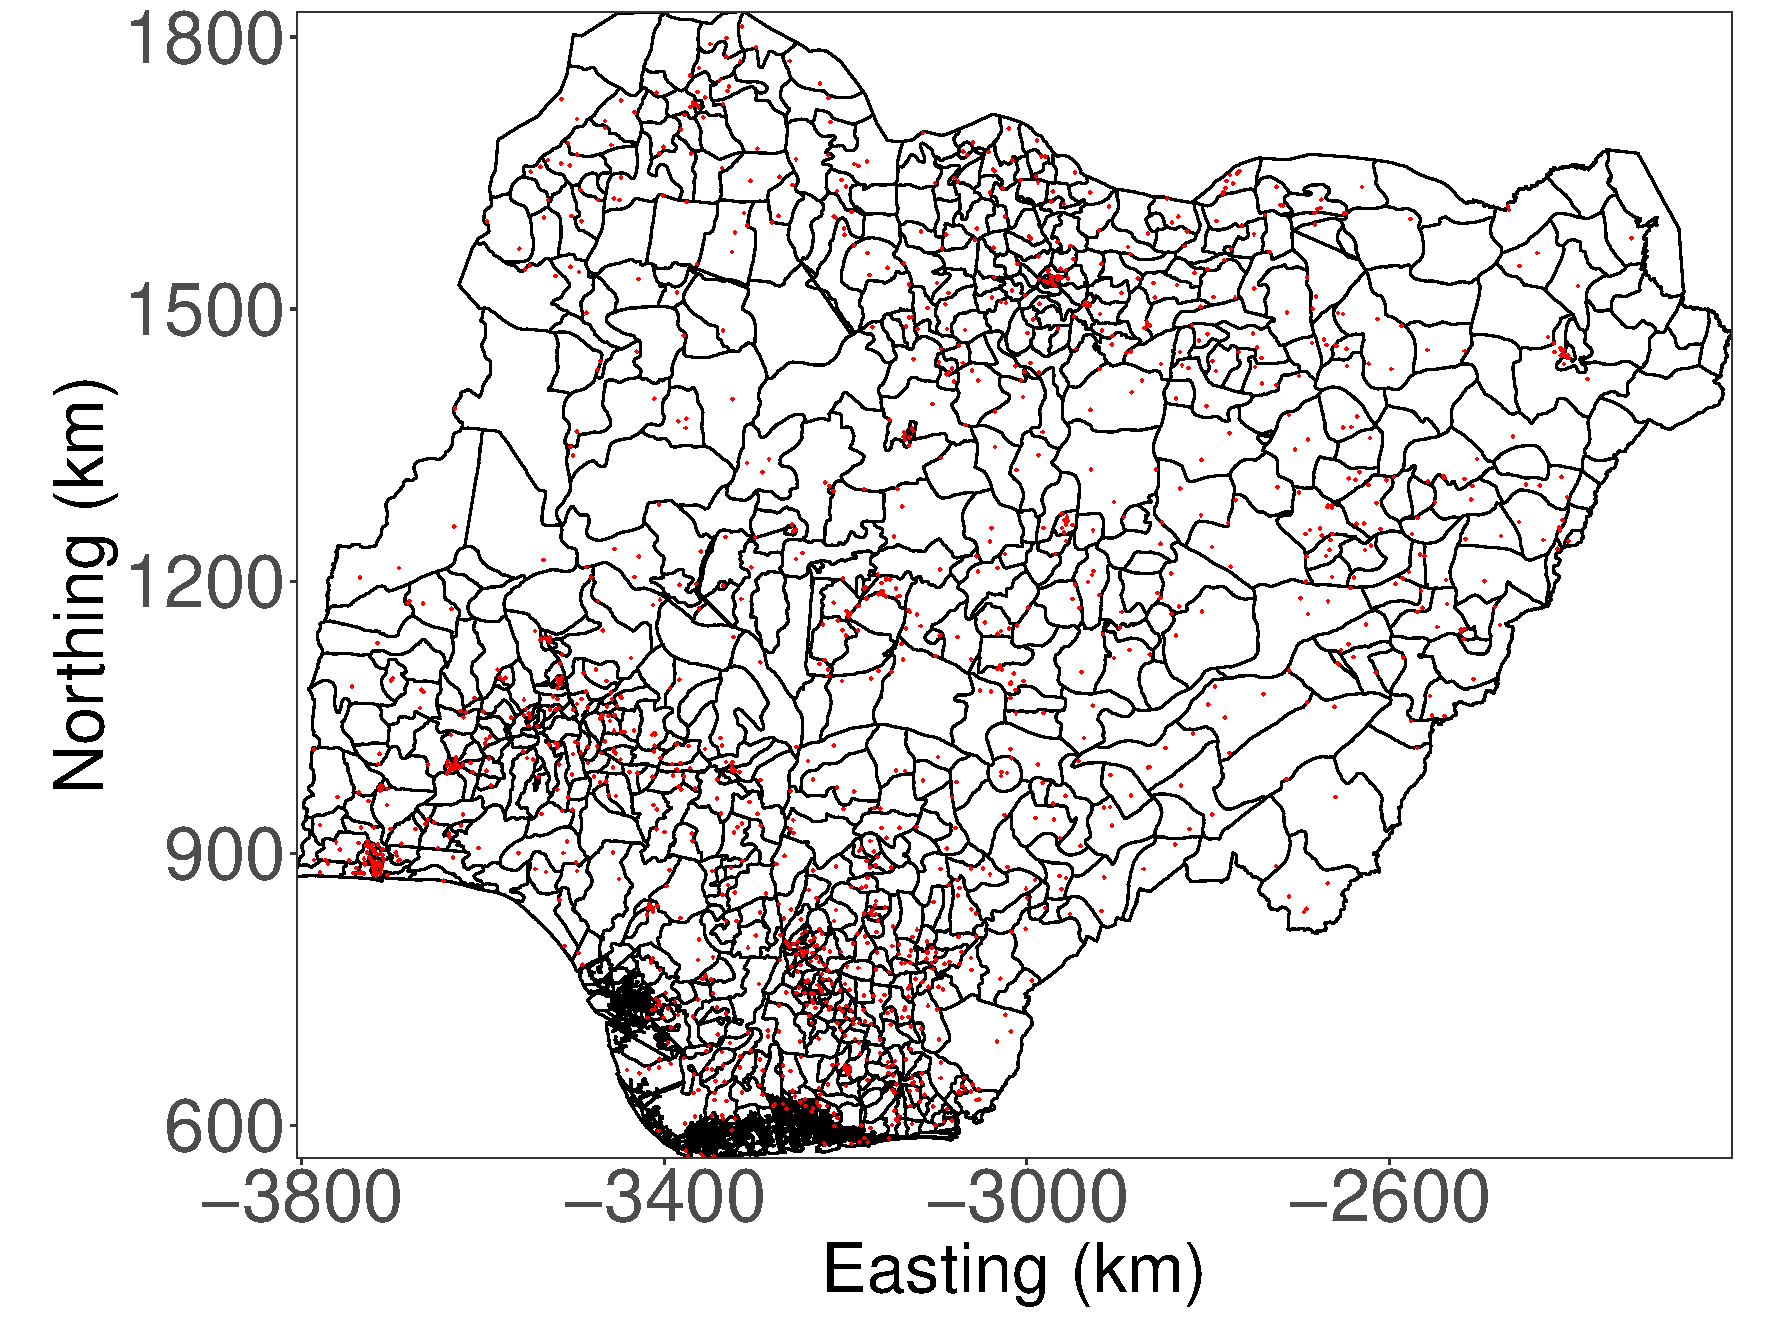
\includegraphics[width=.48\textwidth]{map.pdf}  
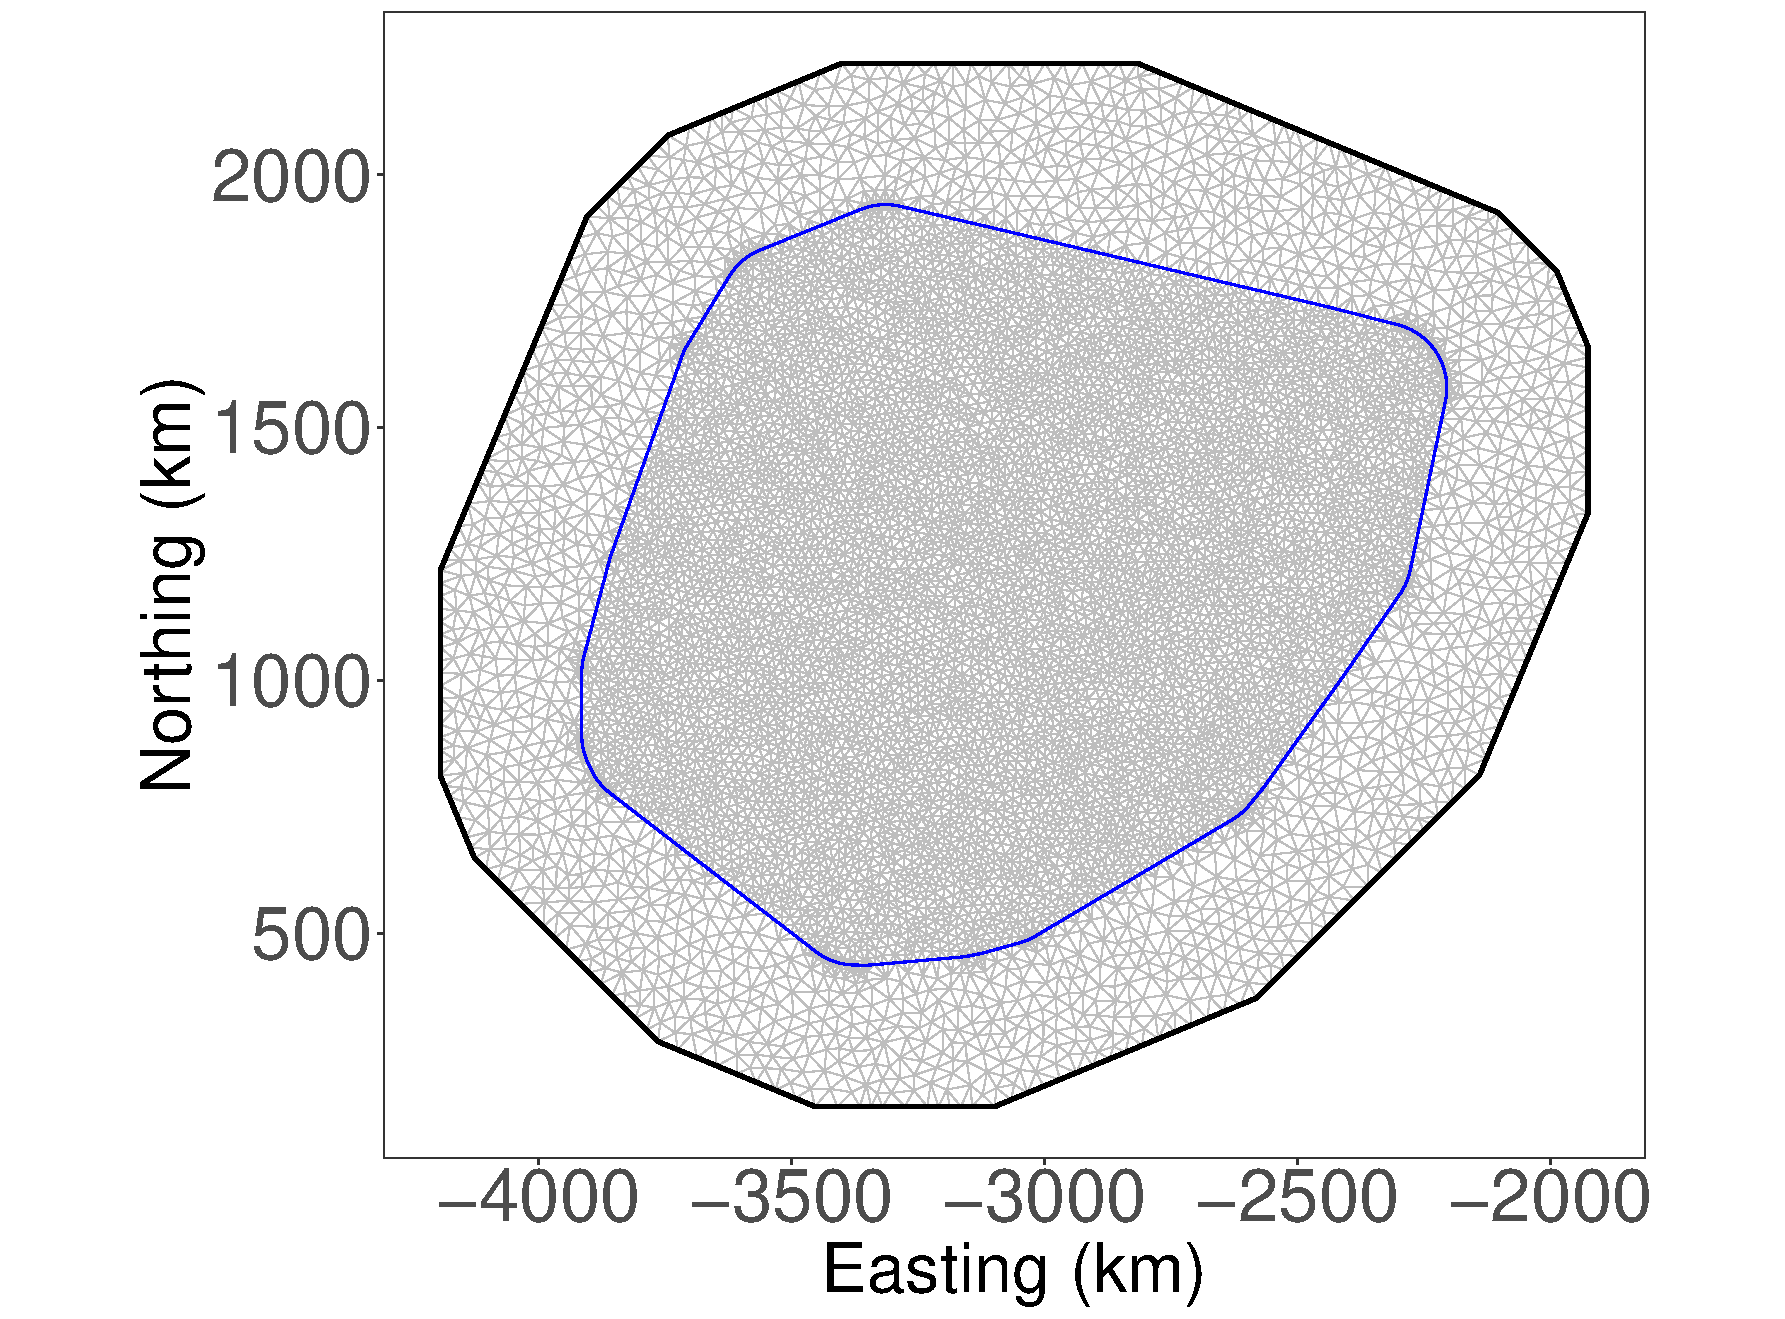
\includegraphics[width=.48\textwidth]{mesh.pdf}
\caption{Nigeria subnational level map (left) and the triangular mesh (right). The red points represent the jittered cluster centers.}
\label{fig:meshAndCountry}
\end{figure}


\begin{example}
# Set target geometry
target_crs = "+units=km +proj=utm +zone=37 +ellps=clrk80 
              +towgs84=-160,-6,-302,0,0,0,0 +no_defs"

# transform admin0 borders into target_crs: 
admin0_trnsfrmd = sf::st_transform(admin0, target_crs)

# construct the mesh
mesh.s = meshCountry(admin0= admin0_trnsfrmd,
                     max.edge = c(25, 50),
                     offset = -.08, cutoff=4,
                     target_crs = target_crs)
\end{example}
%\caption{Input preparation: construct the triangular mesh with the function \code{meshCountry}}
%\label{lst:NigeriaExample5}
%\end{listing}

Figure \ref{fig:meshAndCountry} shows the admin2 borders together with the resulting triangular mesh.
We use the function \code{prepareInput} to collect all data required for estimation and to precompute integration points and integration weights necessary for the method described in the method section.
%\texttt{prepareInput} function uses the model responses to construct response vectors for the corresponding urban and rural integration points. The example in this section uses a binomial model.

\begin{example}
# read the covariate raster
library(terra)
r = terra::rast("Nga_ppp_v2c_2015.tif")

inputData = prepareInput(response=list(ys=nigeria.data$ys,ns=nigeria.data$ns),
                                  locObs = pointsKM, 
                                  likelihood = 1,
                                  urban = nigeria.data$urbanRuralDHS, 
                                  mesh.s = mesh.s, 
                                  adminMap = admin2,
                                  covariateData = list(r), 
                                  target_crs = target_crs)
\end{example}
%\caption{Input preparation: prepare data input for estimation with function \code{prepareInput()}}
%\label{lst:NigeriaExample6}
%\end{listing}


Since the likelihood is binomial, we set the argument \texttt{response} to a list  containing the number of trials \code{ns} and a list of the number of successes \code{ys} for the clusters. Here, \code{ns} is $(n_1, \ldots, n_{1380})^\mathrm{T}$ and \code{ys} is $(y_1, \ldots, y_{1380})^\mathrm{T}$. We pass the covariate \texttt{SpatRaster} objects within a list, through the argument \code{list(terra::rast(r = r))}. 
\CRANpkg{GeoAdjust} allows modelling the data with either one of Gaussian, binomial or Poisson likelihoods. Accordingly, the likelihood type needs to be passed into the function via the argument \texttt{likelihood}, by setting it to either 0, 1 or 2, respectively. We set the binomial likelihood with \code{likelihood = 1}.



\section{Step 2: Estimation}
We estimate the model using the function \code{estimateModel}. 

\begin{example}
# estimating the parameters
est = estimateModel(
      data = inputData, 
      priors = list(beta = c(0,1), range = 114), 
                    USpatial = 1, alphaSpatial = 0.05,
                    UNugget = 1, alphaNug = 0.05,
      n.sims = 1000)
\end{example}
%\caption{Estimation: using the function \code{estimateModel}.}
%\label{lst:NigeriaExample8}
%\end{listing}

Here we set priors $\beta_0, \beta_1 \overset{\text{iid}}{\sim}\mathcal{N}(0, 1)$ using \code{beta = c(0,1)}. We choose the prior on marginal variance $\sigma_\mathrm{S}^2$ such that $\mathrm{P}(\sigma_\mathrm{S} > 1) = 0.05$ through \code{USpatial = 1} and \code{alphaSpatial = 0.05}. We use \code{n.sims = 1000} draws from the estimated posteriors. The median of the prior on range $\rho_\mathrm{S}$ is set to \code{range = 114} km. The function \code{estimateModel} returns a list of four elements: \code{res}, \code{obj}, \code{draws} and \code{likelihood}. 

\begin{example}
# the output of estimateModel() function:
names(est)
[1] "res"        "obj"        "draws"      "likelihood"

print(est)

GeoAdjust::estimateModel() 
----------------------------------
Likelihood :          binomial
----------------------------------
parameter estimate    95% CI length
range     69.7677     NA
sigma     2.1462      NA
intercept -1.2998     0.6578
beta1     0.0069      0.0044
----------------------------------
\end{example}
%\caption{Estimation: output of \code{estimateModel}.}
%\label{lst:NigeriaExample9}
%\end{listing}

The elements \code{obj} and \code{draws} are used for prediction in the next section. The element 
\code{likelihood} indicates the likelihood type (\code{0} is Gaussian, \code{1} is binomial, and \code{2} is Poisson) that is used in the model construction, and \code{res} contains the estimated model parameters and the lengths of 95\% credible intervals. The credible interval lengths are calculated as the difference between the 97.5\%  and 2.5\%  percentiles. The result object \texttt{res} does not contain \code{CI\_Length} values for the range and the marginal variance, as the inference is empirical Bayesian where these parameters are estimated to fixed values.

\section{Step 3: Prediction \label{sec:estPred}} 
We grid the country using the function \code{gridCountry} with  the admin0 boundaries and a resolution of 5 km.

\begin{example}
# raster and the prediction coordinates:
predComponents = gridCountry(admin0 = admin0, 
                             res = 5, 
                             target_crs = target_crs)

names(predComponents)
[1] "loc.pred" "predRast"

# the sf multipoint object containing the prediction locations
loc.pred = predComponents[["loc.pred"]]

> print(loc.pred)
Simple feature collection with 80201 features and 0 fields
Geometry type: POINT
Dimension:     XY
Bounding box:  xmin: -3803.253 ymin: 565.4467 
               xmax: -2223.253 ymax: 1825.447
Projected CRS: +units=km +proj=utm +zone=37 +ellps=clrk80 +towgs84=-160,-6,-302,
0,0,0,0 +no_defs
First 10 features:
                     geometry
1  POINT (-3803.253 1825.447)
2  POINT (-3798.253 1825.447)
3  POINT (-3793.253 1825.447)
4  POINT (-3788.253 1825.447)
5  POINT (-3783.253 1825.447)
6  POINT (-3778.253 1825.447)
7  POINT (-3773.253 1825.447)
8  POINT (-3768.253 1825.447)
9  POINT (-3763.253 1825.447)
10 POINT (-3758.253 1825.447)

predRast = predComponents[["predRast"]]

> print(predRast)
class       : SpatRaster 
dimensions  : 253, 317, 1  (nrow, ncol, nlyr)
resolution  : 5, 5  (x, y)
extent      : -3805.753, -2220.753, 562.9467, 1827.947  
             (xmin, xmax, ymin, ymax)
coord. ref. : +proj=utm +zone=37 +ellps=clrk80 +towgs84=-160,-6,-302,0,0,0,
0 +units=km +no_defs 
\end{example}
%\caption{Prediction: the \texttt{gridCountry()} function.}
%\label{lst:NigeriaExample10}
%\end{listing}

The output shows that the grid cell centroids are 5 km apart and the dimension of the grid is $253 \times 317$. This includes locations that are outside the admin0 boundaries, which will be masked when plotting the predictions.


We use the function \code{predRes} with \code{flag = 1} to indicate the Binomial likelihood, and that the inverse of the logit needs to be applied to the linear predictor. The argument \code{covariateData} contains a list of one element which is the population density raster. Additionally, we input the objects \code{obj} and \code{draws} from the function \code{estimateModel}. 

\begin{example}
predictions = predRes(obj = est[["obj"]] , predCoords = loc.pred,
                      draws = est[["draws"]],
                      covariateData = list(r),
                      mesh.s = mesh.s, flag = 1)

head(predictions)
          mean    median         sd       lower     upper
[1,] 0.2155746 0.2143489 0.02934076 0.165192003 0.2764130
[2,] 0.3471947 0.2220279 0.33308573 0.001691273 0.9860286
[3,] 0.3442247 0.2269676 0.32558640 0.002292870 0.9839695
[4,] 0.3447684 0.2402942 0.32414517 0.001921544 0.9817542
[5,] 0.3379962 0.2405484 0.31493574 0.002677005 0.9755113
[6,] 0.3329591 0.2317648 0.30754117 0.003479042 0.9637670

dim(predictions)
[1] 80201     5
\end{example}
%\caption{Prediction: the \texttt{predRes()} function.}
%\label{lst:NigeriaExample11}
%\end{listing}
 
The result object contains the desired quantities for each grid cell in Nigeria. We use the function \code{plotPred} to plot the predictions and the corresponding uncertainty accross the studied country. The uncertainty is quantified as the coefficient of variation (CV), which is calculated as $\frac{\sigma}{\mu} \times 100$, where $\sigma$ and $\mu$ is the standard deviation and mean, respectively, of the predictive distribution.

\begin{example}
admin1 = st_read("gadm40_NGA_shp/gadm40_NGA_1.shp")
                 
plotPred(pred = predictions, 
         predRaster = predRast, 
         admin0 = admin0,
         admin1 = admin1, 
         admin2 = admin2, 
         rmPoly = 160,
         target_crs = target_crs)
\end{example}
%\caption{Prediction: plotting.}
%\label{lst:NigeriaExample12}
%\end{listing}

%The first argument \texttt{pred} is the output of the function  \texttt{predRes} which is obtained in Listing~\ref{lst:NigeriaExample11}. 
Here we provide \code{predRaster}, which is the locations and geography for prediction, and the predicted values \code{pred}.
%The arguments \texttt{admin0}, \texttt{admin1} and \texttt{admin2} refer to the \texttt{sf} class \texttt{MULTIPOLYGON} objects representing the national, and the first and second level subnational administrative borders of the corresponding country.
The argument \code{admin0} is used to mask values outside Nigeria, the argument \code{admin1} is used to plot the first administrative level (admin1) borders, and the argument \code{admin2} together with \code{rmPoly = 160} is used to remove the admin2 area corresponding to the lake, which is not a real admin2 area, from plotting. The arguments \texttt{rmPoly} and \texttt{admin2} should be set to \texttt{NULL} if all admin2 areas should be plotted. 
%The argument \texttt{locObs}, as an \texttt{sf} \texttt{POINT} object, indicates the observed locations, or in other words, the DHS cluster centers. The function plots these as red dots on to the map. 
Figure \ref{fig:predPlot} shows the resulting predictions and CVs.  The function returns a list containing two \texttt{ggplot} objects, representing the plots for the predictions and uncertainty across the country of interest. 


%Figure \ref{fig:predPlot} shows the predicted risk and the corresponding uncertainty across Nigeria. Please note that since we assigned "\texttt{NA}" to the points that overlap with the lake, the north-east corner of the plots are not colored. This area is the area covered by the lake. This is specific to the geography of Nigeria and different features like this may need to be considered while plotting data on the maps of different countries.

\begin{figure}
\centering
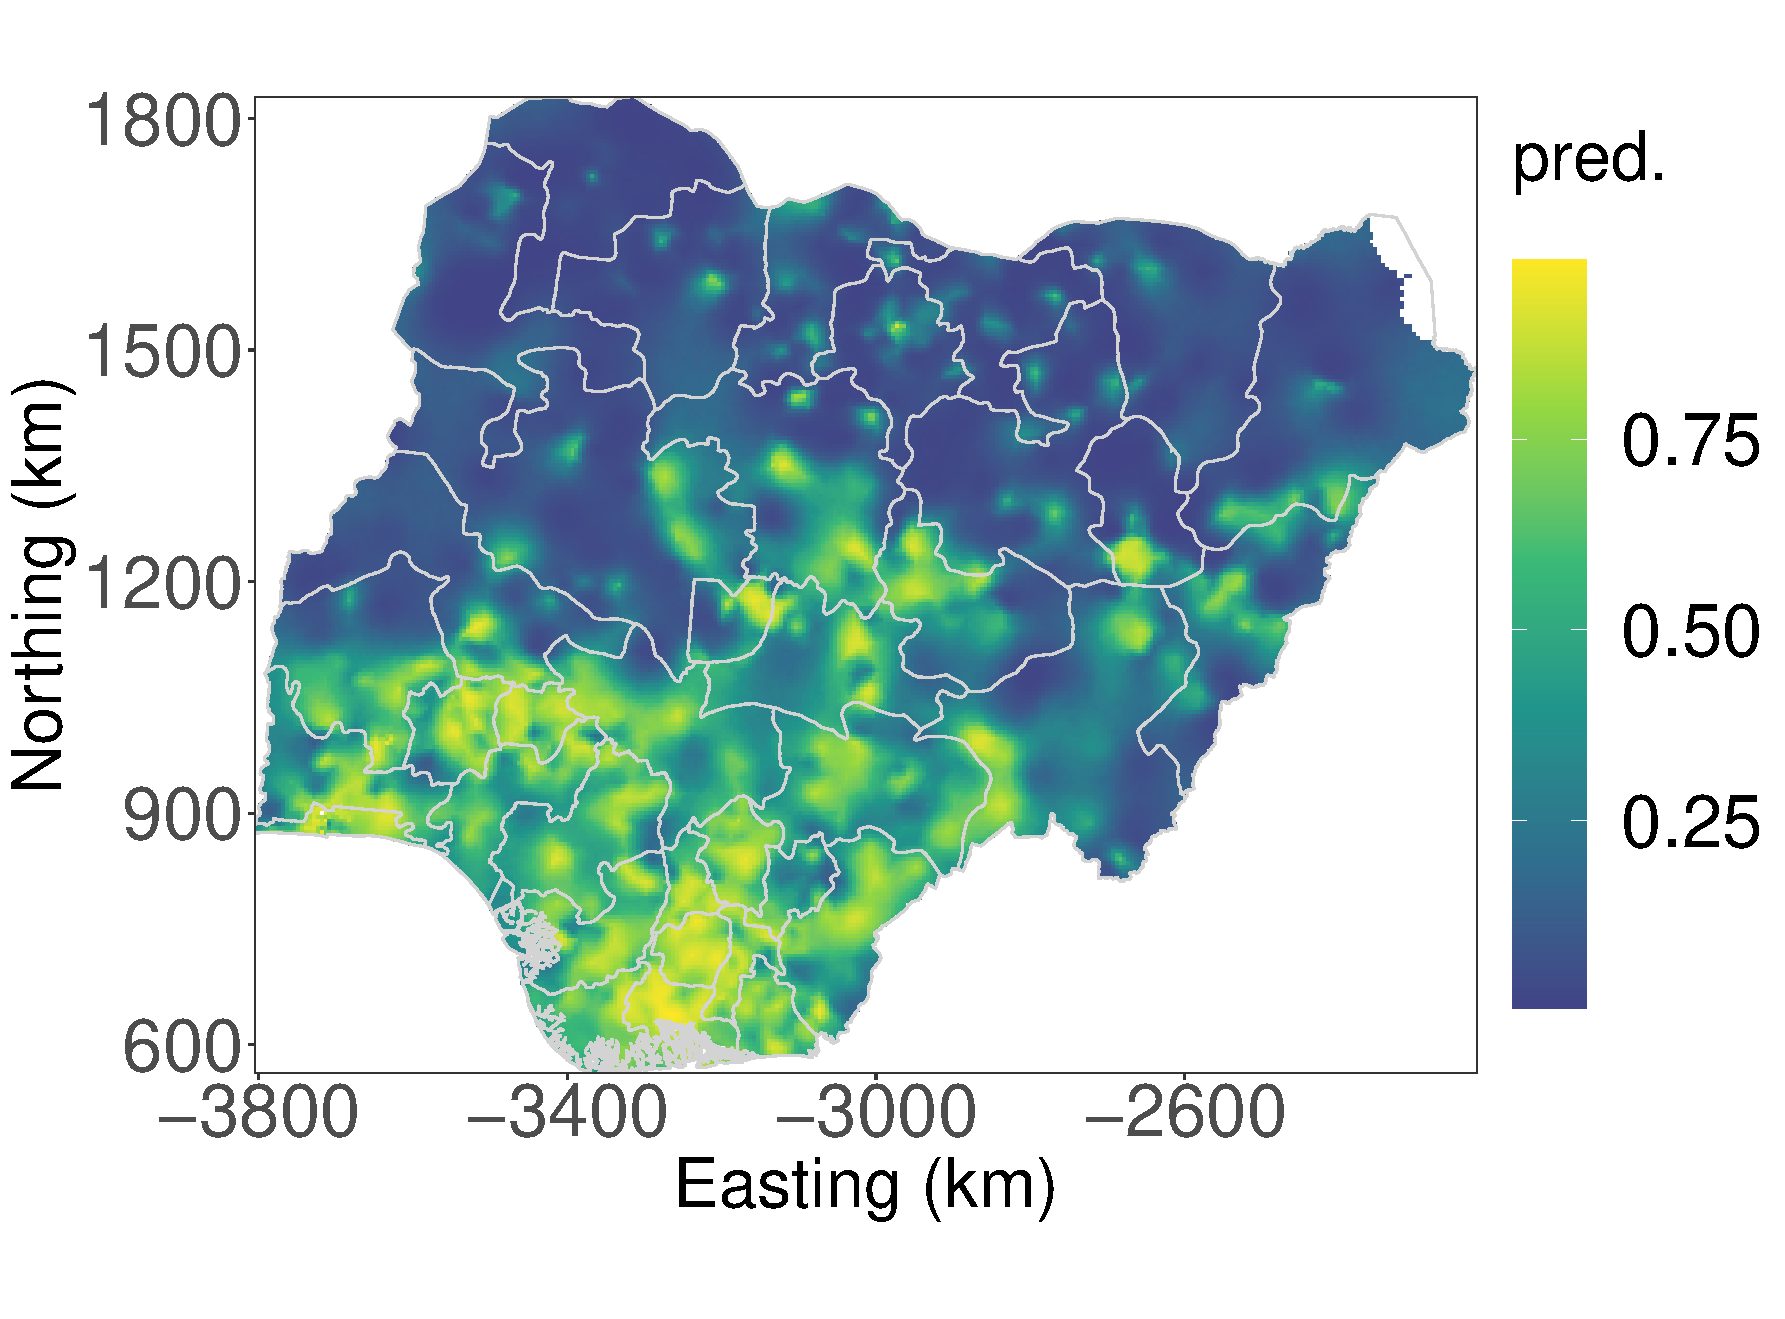
\includegraphics[height=4.8cm]{pred.pdf} \hspace{.005 \textwidth} 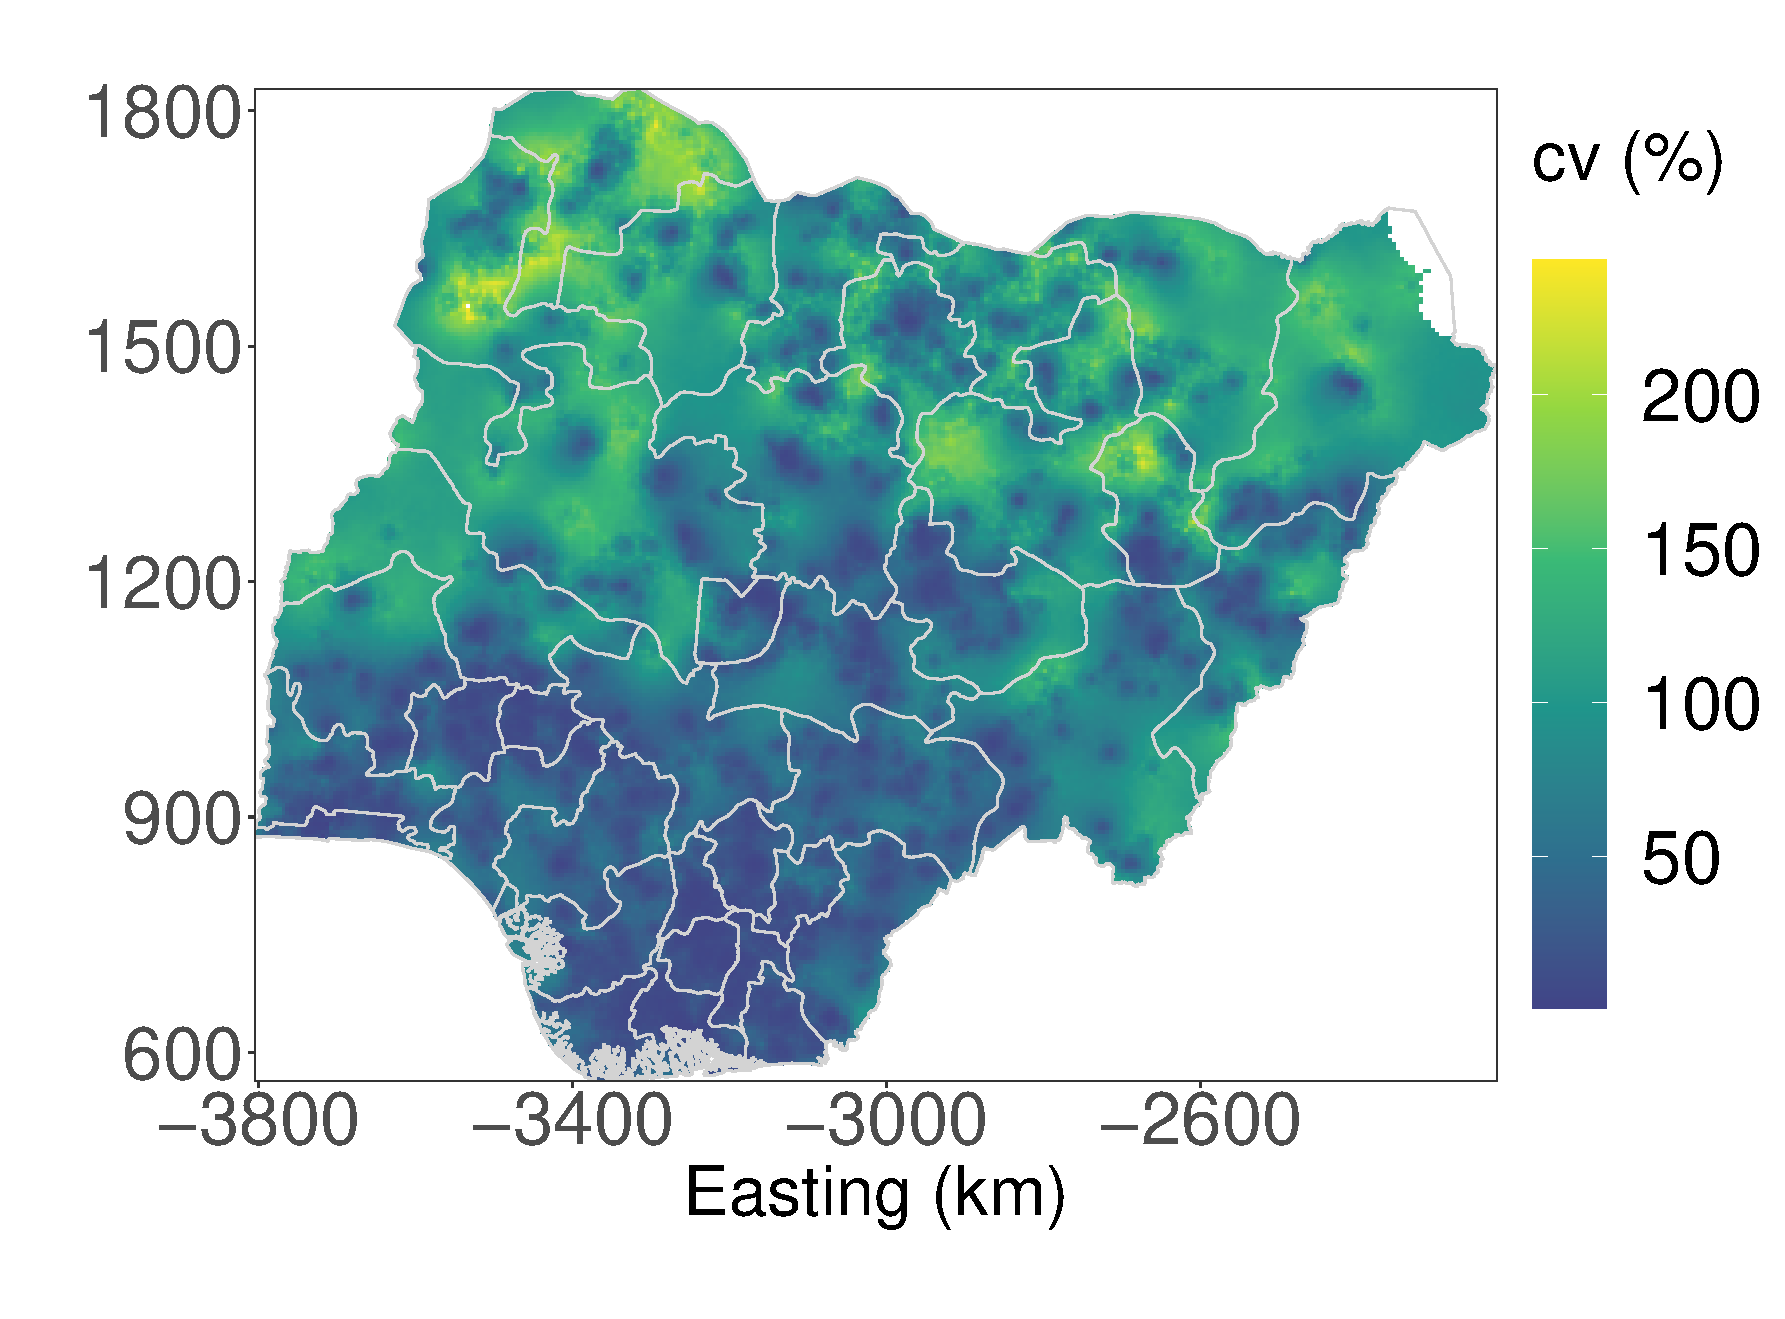
\includegraphics[height=4.8cm]{uncertainty.pdf}
\caption{Predicted risk (left) and the CVs (right). The red points indicate the example survey cluster centers.}
\label{fig:predPlot}
\end{figure}


\section{Summary}
\CRANpkg{GeoAdjust} allows fast and easy geostatistical analysis of DHS household survey data while accounting for jittering. The user can take advantage of a novel complex method \citep{altay2022accounting,altay2022covariates} and control settings without being exposed to complex code. The user also has access to convenient plotting functions, and the backend uses \CRANpkg{sf} and \CRANpkg{terra} to handle spatial data with information on coordinate systems and rasters. \CRANpkg{GeoAdjust} is the only package that  addresses the positional uncertainty in DHS data, and has the potential to be extended to combine  areal and point referenced data from different areas involving the both positional uncertainty and geomasking.



\bibliography{references.bib}

\address{%
Umut Altay\\
Department of Mathematical Sciences, Norwegian University of Science and Technology\\%
Trondheim, Norway\\
%
%
%
\href{mailto:umut.altay@ntnu.no}{\nolinkurl{umut.altay@ntnu.no}}%
}

\address{%
John Paige\\
Department of Mathematical Sciences, Norwegian University of Science and Technology\\%
Trondheim, Norway\\
%
%
%
\href{mailto:john.paige@ntnu.no}{\nolinkurl{john.paige@ntnu.no}}%
}

\address{%
Andrea Riebler\\
Department of Mathematical Sciences, Norwegian University of Science and Technology\\%
Trondheim, Norway\\
%
%
%
\href{mailto:andrea.riebler@ntnu.no}{\nolinkurl{andrea.riebler@ntnu.no}}%
}

\address{%
Geir-Arne Fuglstad\\
Department of Mathematical Sciences, Norwegian University of Science and Technology\\%
Trondheim, Norway\\
%
%
%
\href{mailto:geir-arne.fuglstad@ntnu.no}{\nolinkurl{geir-arne.fuglstad@ntnu.no}}%
}
